% !TeX program = xelatex
\documentclass[a4paper,10pt]{article}

% ============================================================================
% កញ្ចប់បណ្ណាល័យ (Packages) – អនុវិទ្យាល័យព្រះក្រសាំង (គ្មាន LCD / សន្លឹកកិច្ចការជាគោល)
% ============================================================================
\usepackage[a4paper, left=0.95cm, right=0.95cm, top=0.85cm, bottom=0.92cm, footskip=0.52cm]{geometry}
\usepackage{amsmath}
\usepackage{unicode-math}
\usepackage{fontspec}
\usepackage{array, longtable, multirow, colortbl}
\usepackage[table]{xcolor}
\usepackage{enumitem}
\usepackage{pifont}
\usepackage{fancyhdr}
\usepackage{tikz}
\usetikzlibrary{calc, arrows.meta, decorations.pathreplacing, patterns, positioning, babel}

\makeatletter
\let\@expl@@@mark@update@singlecol@structures@@\relax
\makeatother

% ============================================================================
% ការកំណត់ពុម្ពអក្សរ (Cross-Platform Windows + Linux Cloud fonts/)
% ============================================================================
\providecommand{\NGSFindFonts}{%
  \IfFileExists{C:/Windows/Fonts/cambria.ttc}{%
    \def\NGSSysPath{C:/Windows/Fonts/}%
    \def\NGSUserPath{C:/Users/KIT/AppData/Local/Microsoft/Windows/Fonts/}%
  }{%
    \IfFileExists{./fonts/KhmerOSsiemreap.ttf}{\def\NGSSysPath{./fonts/}\def\NGSUserPath{./fonts/}}{%
    \IfFileExists{../fonts/KhmerOSsiemreap.ttf}{\def\NGSSysPath{../fonts/}\def\NGSUserPath{../fonts/}}{%
    \IfFileExists{../../fonts/KhmerOSsiemreap.ttf}{\def\NGSSysPath{../../fonts/}\def\NGSUserPath{../../fonts/}}{%
    \IfFileExists{../../../fonts/KhmerOSsiemreap.ttf}{\def\NGSSysPath{../../../fonts/}\def\NGSUserPath{../../../fonts/}}{%
    \IfFileExists{../../../../fonts/KhmerOSsiemreap.ttf}{\def\NGSSysPath{../../../../fonts/}\def\NGSUserPath{../../../../fonts/}}{%
    \IfFileExists{../../../../../fonts/KhmerOSsiemreap.ttf}{\def\NGSSysPath{../../../../../fonts/}\def\NGSUserPath{../../../../../fonts/}}{%
    \IfFileExists{../../../../../../fonts/KhmerOSsiemreap.ttf}{\def\NGSSysPath{../../../../../../fonts/}\def\NGSUserPath{../../../../../../fonts/}}{%
      \def\NGSSysPath{../../../../../../../fonts/}\def\NGSUserPath{../../../../../../../fonts/}%
    }}}}}}}%
  }%
}
\NGSFindFonts

\setmathfont[
  Path={\NGSSysPath},
  FontIndex=1,
  Scale=1.02
]{cambria.ttc}

\defaultfontfeatures{Ligatures=TeX}

\setmainfont[
  Path={\NGSUserPath},
  Extension=.ttf,
  Script=Khmer,
  BoldFont={KhmerOSsiemreap},
  BoldFeatures={FakeBold=1.8},
  ItalicFont={KhmerOSsiemreap},
  ItalicFeatures={FakeSlant=0.25},
  BoldItalicFont={KhmerOSsiemreap},
  BoldItalicFeatures={FakeBold=1.8, FakeSlant=0.25}
]{KhmerOSsiemreap}

\newfontfamily\muol[
  Path={\NGSUserPath},
  Extension=.ttf,
  Script=Khmer
]{KhmerOSmuollight}

\newfontfamily\TimesEn[
  Path={\NGSSysPath},
  Extension=.ttf,
  Scale=1.00,
  BoldFont={timesbd},
  ItalicFont={timesi},
  BoldItalicFont={timesbi}
]{times}

\newfontfamily\NagaBold[
  Path={\NGSUserPath},
  Extension=.ttf
]{AKbalthom Naga Bold}

\newfontfamily\CalibriFont[
  Path={\NGSSysPath},
  Extension=.ttf
]{calibri}

\newfontfamily\Tacteing[
  Path={\NGSUserPath}
]{TACTENG.TTF}

\newfontfamily\CourierBullet[
  Path={\NGSSysPath},
  Extension=.ttf
]{cour}
\newcommand{\wcirc}{{\CourierBullet\fontsize{9.5pt}{11pt}\selectfont o}}

\XeTeXlinebreaklocale "km"
\XeTeXlinebreakskip = 0pt plus 1pt minus 0.1pt

% ============================================================================
% ការកំណត់ពណ៌ និងទម្រង់ទំព័រ (Colors & Page Style)
% ============================================================================
\definecolor{stepgray}{HTML}{D9D9D9}
\definecolor{headgray}{HTML}{F2F2F2}
\definecolor{boxgray}{HTML}{D9D9D9}
\definecolor{darkred}{HTML}{C00000}
\definecolor{red5e}{HTML}{FF0000}

\pagestyle{fancy}
\fancyhf{}
\renewcommand{\headrulewidth}{0pt}
\fancyfoot[R]{\CalibriFont\fontsize{11pt}{13pt}\selectfont\thepage}

\setlength{\parindent}{0pt}
\setlength{\parskip}{0pt}
\setlength{\tabcolsep}{3.8pt}

\newcolumntype{L}[1]{>{\raggedright\arraybackslash}p{#1}}

% ============================================================================
% ម៉ាក្រូជំនួយ (Helper Macros)
% ============================================================================
\newcommand{\en}[1]{{\TimesEn #1}}
\newcommand{\enbf}[1]{{\TimesEn\textbf{#1}}}
\newcommand{\unit}[1]{\,\text{\en{#1}}}
\newcommand{\riel}{\,\text{៛}}
\newcommand{\fiveE}[1]{{\NagaBold\fontsize{9.5pt}{13pt}\selectfont\textcolor{red5e}{#1}}}
\newcommand{\timenote}[1]{\textcolor{darkred}{\textit{#1}}}
\newcommand{\redsub}[1]{\textcolor{darkred}{#1}}
\newcommand{\graybox}[1]{\colorbox{boxgray}{\strut\hspace{2pt}#1\hspace{2pt}}}
\newcommand{\ditem}{\tikz[baseline=-0.5ex]\fill (0,0.42ex) -- (0.42ex,0) -- (0,-0.42ex) -- (-0.42ex,0) -- cycle;\hspace{0.3em}}
\newcommand{\cnum}[1]{{\fontsize{10.5pt}{12pt}\selectfont\ding{\numexpr181+#1\relax}}\hspace{0.15em}}
\newcommand{\cfig}[1]{\par\vspace{3pt}{\centering #1\par}\vspace{3pt}}
\newcommand{\stepheader}[1]{\multicolumn{3}{|c|}{\cellcolor{stepgray}\muol #1} \\* \noalign{\hrule height 0.4pt}}
\newcommand{\fboxb}[1]{\begingroup\setlength{\fboxsep}{1.5pt}\fbox{#1}\endgroup}
\newcommand{\khmflourish}{{\Tacteing\fontsize{36pt}{14pt}\selectfont\raisebox{-5pt}{3}}}

% ============================================================================
% ម៉ាក្រូគូសរូប TikZ ស-ខ្មៅ ១០០% (x=1cm, y=1cm, font=\scriptsize, width=7.55cm)
% ============================================================================

% ១. E1 Engage: ពង្រីករូបថតសមាមាត្រ & ចែកអង្ករសង្គ្រោះទឹកជំនន់
\newcommand{\figEngagePROPThreeOneTwo}{%
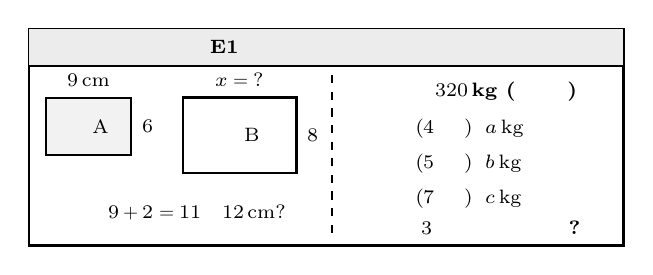
\begin{tikzpicture}[x=1cm, y=1cm, every node/.style={font=\scriptsize, text=black}]
  \draw[black, line width=0.9pt] (0,0) rectangle (7.55,2.75);
  \fill[gray!15] (0,2.28) rectangle (7.55,2.75);
  \draw[black, line width=0.6pt] (0,2.28) -- (7.55,2.28);
  \node at (3.775,2.515) {\textbf{បេសកកម្ម \en{E1}៖ ពង្រីករូបថតសិស្ស និងចែកអង្ករសង្គ្រោះទឹកជំនន់}};

  % ឆ្វេង៖ រូបថត 2 សន្លឹក
  \draw[black, line width=0.8pt, fill=gray!10] (0.22,1.15) rectangle (1.30,1.87);
  \node at (0.76,1.51) {រូប \en{A}};
  \node[above=0.5pt] at (0.76,1.87) {$9\unit{cm}$};
  \node[right=0.5pt] at (1.30,1.51) {$6$};

  \draw[black, line width=0.85pt] (1.96,0.92) rectangle (3.40,1.88);
  \node at (2.68,1.40) {រូប \en{B}};
  \node[above=0.5pt] at (2.68,1.88) {$x = ?$};
  \node[right=0.5pt] at (3.40,1.40) {$8$};
  \node at (1.88,0.42) {ស្មាន៖ $9+2=11$ ឬ $12\unit{cm}$?};

  \draw[black, line width=0.6pt, dashed] (3.85,0.16) -- (3.85,2.18);

  % ស្ដាំ៖ អង្ករ 320 kg សម្រាប់ 3 គ្រួសារ (4, 5, 7 នាក់)
  \node at (5.70,1.95) {\textbf{អង្ករសរុប $320\unit{kg}$ (៣ គ្រួសារ)}};
  \node[anchor=west] at (4.00,1.48) {គ្រួសារទី១ ($4$ នាក់)៖ $a\unit{kg}$};
  \node[anchor=west] at (4.00,1.04) {គ្រួសារទី២ ($5$ នាក់)៖ $b\unit{kg}$};
  \node[anchor=west] at (4.00,0.60) {គ្រួសារទី៣ ($7$ នាក់)៖ $c\unit{kg}$};
  \node at (5.70,0.22) {\textbf{ចែកស្មើ $3$ គ្រួសារ ឬតាមចំនួនមនុស្ស?}};
\end{tikzpicture}}

% ២. E2 Act 1: លក្ខណៈទី 1 គូសព្រួញខ្វែងតួចុង-តួមធ្យម [X-trace] (ទំ.២៨)
\newcommand{\figExploreCrossPROPThreeOneTwo}{%
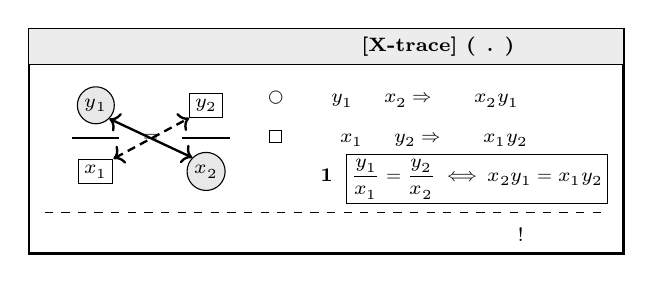
\begin{tikzpicture}[x=1cm, y=1cm, every node/.style={font=\scriptsize, text=black}]
  \draw[black, line width=0.9pt] (0,0) rectangle (7.55,2.85);
  \fill[gray!15] (0,2.40) rectangle (7.55,2.85);
  \draw[black, line width=0.6pt] (0,2.40) -- (7.55,2.40);
  \node at (3.775,2.625) {\textbf{សកម្មភាព ១៖ ព្រួញខ្វែងតួចុង និងតួមធ្យម \en{[X-trace]} (ទំ.២៨)}};

  % សមាមាត្រខាងឆ្វេង
  \node[draw=black, circle, inner sep=1.5pt, fill=gray!18] (Y1) at (0.85,1.88) {$y_1$};
  \draw[black, line width=0.8pt] (0.55,1.46) -- (1.15,1.46);
  \node[draw=black, rectangle, inner sep=2pt, fill=white] (X1) at (0.85,1.04) {$x_1$};

  \node at (1.55,1.46) {$=$};

  \node[draw=black, rectangle, inner sep=2pt, fill=white] (Y2) at (2.25,1.88) {$y_2$};
  \draw[black, line width=0.8pt] (1.95,1.46) -- (2.55,1.46);
  \node[draw=black, circle, inner sep=1.5pt, fill=gray!18] (X2) at (2.25,1.04) {$x_2$};

  % ព្រួញខ្វែង
  \draw[black, line width=0.85pt, <->] (Y1.south east) -- (X2.north west);
  \draw[black, line width=0.85pt, densely dashed, <->] (X1.north east) -- (Y2.south west);

  % ការពន្យល់ខាងស្ដាំ
  \node[anchor=west] at (2.92,1.96) {$\bigcirc$ \textbf{តួចុង៖} $y_1$ និង $x_2 \Rightarrow$ ផលគុណ $x_2 y_1$};
  \node[anchor=west] at (2.92,1.46) {{\fboxsep=0pt\fbox{\rule{0pt}{1.35ex}\hspace{1.35ex}}} \textbf{តួមធ្យម៖} $x_1$ និង $y_2 \Rightarrow$ ផលគុណ $x_1 y_2$};
  \node[anchor=west] at (2.92,0.94) {\textbf{លក្ខណៈទី 1៖} \fboxb{$\dfrac{y_1}{x_1} = \dfrac{y_2}{x_2} \iff x_2 y_1 = x_1 y_2$}};

  \draw[black, line width=0.55pt, dashed] (0.20,0.52) -- (7.35,0.52);
  \node at (3.775,0.24) {\textbf{វិន័យតម្រៀបជួរ៖} ភាគយកដាក់ខ្នាតដូចគ្នា ភាគបែងដាក់ខ្នាតដូចគ្នាមុនគុណខ្វែង!};
\end{tikzpicture}}

% ៣. E2 Act 2: POE ញែកសញ្ញា '=' (លក្ខណៈទី 2) ពីសញ្ញា '+' (អន្ទាក់បូកប្រភាគខុសក្បួន)
\newcommand{\figPOESumPROPThreeOneTwo}{%
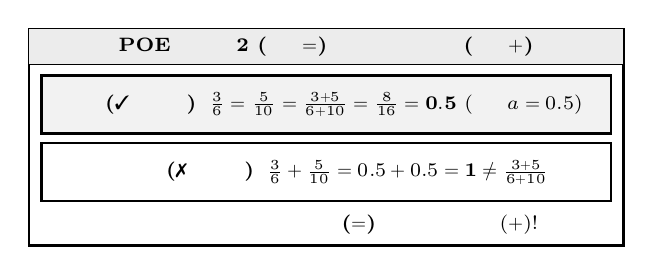
\begin{tikzpicture}[x=1cm, y=1cm, every node/.style={font=\scriptsize, text=black}]
  \draw[black, line width=0.9pt] (0,0) rectangle (7.55,2.75);
  \fill[gray!15] (0,2.30) rectangle (7.55,2.75);
  \draw[black, line width=0.6pt] (0,2.30) -- (7.55,2.30);
  \node at (3.775,2.525) {\textbf{\en{POE}៖ លក្ខណៈទី 2 (សញ្ញា $=$) ធៀបនឹងអន្ទាក់បូកប្រភាគ (សញ្ញា $+$)}};

  % ជួរលើ៖ លក្ខណៈទី 2 ត្រូវ
  \draw[black, line width=0.85pt, fill=gray!10] (0.16,1.42) rectangle (7.39,2.16);
  \node at (3.775,1.79) {\textbf{ត្រូវ (\ding{51} ផលធៀបស្មើ)៖} $\frac{3}{6} = \frac{5}{10} = \frac{3+5}{6+10} = \frac{8}{16} = \mathbf{0.5}$ (រក្សា $a=0.5$)};

  % ជួរក្រោម៖ អន្ទាក់បូកប្រភាគខុស
  \draw[black, line width=0.8pt] (0.16,0.56) rectangle (7.39,1.30);
  \node at (3.775,0.93) {\textbf{អន្ទាក់ខុស (\ding{55} បូកប្រភាគ)៖} $\frac{3}{6} + \frac{5}{10} = 0.5 + 0.5 = \mathbf{1} \neq \frac{3+5}{6+10}$};

  \node at (3.775,0.26) {\textbf{សន្និដ្ឋាន៖} ប្រើបានតែចំពោះ\textbf{ប្រភាគស្មើគ្នា ($=$)} ហាមប្រើលើផលបូកប្រភាគ ($+$)!};
\end{tikzpicture}}

% ៤ក. E4 Elaborate Model 1: ចតុកោណកែង A, B, C សមាមាត្រ 3:2 (ទំ.២៩)
\newcommand{\figElaborateRectPROPThreeOneTwo}{%
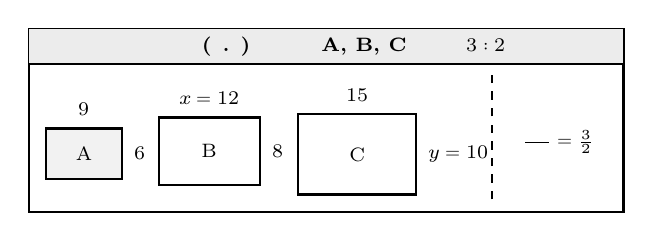
\begin{tikzpicture}[x=1cm, y=1cm, every node/.style={font=\scriptsize, text=black}]
  \draw[black, line width=0.9pt] (0,0) rectangle (7.55,2.32);
  \fill[gray!15] (0,1.88) rectangle (7.55,2.32);
  \draw[black, line width=0.6pt] (0,1.88) -- (7.55,1.88);
  \node at (3.775,2.10) {\textbf{គំរូទី ១ (ទំ.២៩)៖ ចតុកោណកែង \en{A, B, C} សមាមាត្រ $3:2$}};

  \draw[black, line width=0.8pt, fill=gray!10] (0.22,0.42) rectangle (1.18,1.06);
  \node at (0.70,0.74) {\en{A}};
  \node[above=1pt] at (0.70,1.06) {$9$};
  \node[right=1pt] at (1.18,0.74) {$6$};

  \draw[black, line width=0.8pt] (1.65,0.34) rectangle (2.93,1.20);
  \node at (2.29,0.77) {\en{B}};
  \node[above=1pt] at (2.29,1.20) {$x=12$};
  \node[right=1pt] at (2.93,0.77) {$8$};

  \draw[black, line width=0.8pt] (3.42,0.22) rectangle (4.92,1.24);
  \node at (4.17,0.73) {\en{C}};
  \node[above=1pt] at (4.17,1.24) {$15$};
  \node[right=1pt] at (4.92,0.73) {$y=10$};

  \draw[black, line width=0.6pt, dashed] (5.88,0.16) -- (5.88,1.76);
  \node[align=center] at (6.72,0.96) {ផលធៀប\\[2pt]$\frac{\text{បណ្ដោយ}}{\text{ទទឹង}} = \frac{3}{2}$};
\end{tikzpicture}}

% ៤ខ. E4 Elaborate Model 2: គំនូសតាងរបារចំណែករួម 4+5+7=16 (ទំ.៣០)
\newcommand{\figElaborateStripPROPThreeOneTwo}{%
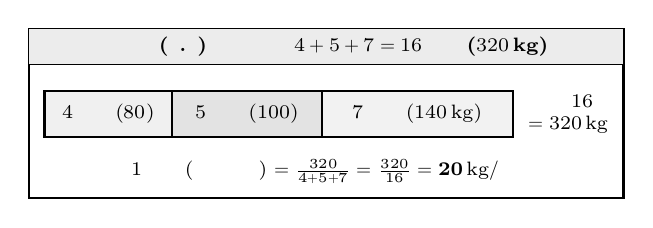
\begin{tikzpicture}[x=1cm, y=1cm, every node/.style={font=\scriptsize, text=black}]
  \draw[black, line width=0.9pt] (0,0) rectangle (7.55,2.15);
  \fill[gray!15] (0,1.70) rectangle (7.55,2.15);
  \draw[black, line width=0.6pt] (0,1.70) -- (7.55,1.70);
  \node at (3.775,1.925) {\textbf{គំរូទី ២ (ទំ.៣០)៖ របារចំណែករួម $4 + 5 + 7 = 16$ ចំណែក ($320\unit{kg}$)}};

  \fill[gray!12] (0.20,0.78) rectangle (1.82,1.36);
  \fill[gray!22] (1.82,0.78) rectangle (3.72,1.36);
  \fill[gray!10] (3.72,0.78) rectangle (6.15,1.36);
  \draw[black, line width=0.85pt] (0.20,0.78) rectangle (6.15,1.36);
  \draw[black, line width=0.75pt] (1.82,0.78) -- (1.82,1.36);
  \draw[black, line width=0.75pt] (3.72,0.78) -- (3.72,1.36);
  \node at (1.01,1.07) {$4$ ចំណែក ($80$)};
  \node at (2.77,1.07) {$5$ ចំណែក ($100$)};
  \node at (4.935,1.07) {$7$ ចំណែក ($140\unit{kg}$)};
  \node[align=center] at (6.85,1.07) {សរុប $16$\\$=320\unit{kg}$};
  \node at (3.775,0.34) {$1$ ចំណែក (មនុស្សម្នាក់) $= \frac{320}{4+5+7} = \frac{320}{16} = \mathbf{20}\unit{kg}/\text{នាក់}$};
\end{tikzpicture}}

% ៥. E5 Evaluate: ជម្រើសវិនិច្ឆ័យ A-D
\newcommand{\figExitPROPThreeOneTwo}{%
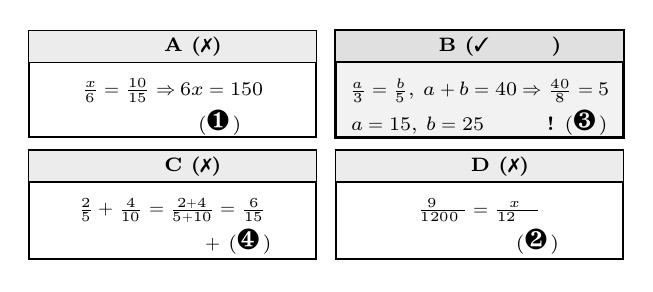
\begin{tikzpicture}[x=1cm, y=1cm, every node/.style={font=\scriptsize, text=black}]
  % A
  \draw[black, line width=0.8pt] (0,1.55) rectangle (3.65,2.90);
  \fill[gray!15] (0,2.50) rectangle (3.65,2.90);
  \draw[black, line width=0.55pt] (0,2.50) -- (3.65,2.50);
  \node at (1.825,2.70) {\textbf{ជម្រើស \en{A} (\ding{55})}};
  \node at (1.825,2.14) {$\frac{x}{6} = \frac{10}{15} \Rightarrow 6x = 150$};
  \node at (1.825,1.74) {គុណចំហៀងខុសក្បួន (\cnum{1})};

  % B (Correct)
  \draw[black, line width=1.1pt, fill=gray!10] (3.90,1.55) rectangle (7.55,2.90);
  \fill[gray!24] (3.90,2.50) rectangle (7.55,2.90);
  \draw[black, line width=0.6pt] (3.90,2.50) -- (7.55,2.50);
  \node at (5.725,2.70) {\textbf{ជម្រើស \en{B} (\ding{51} ត្រឹមត្រូវ)}};
  \node at (5.725,2.14) {$\frac{a}{3}=\frac{b}{5},\; a+b=40 \Rightarrow \frac{40}{8}=5$};
  \node at (5.725,1.74) {\textbf{$a=15,\; b=25$ ត្រឹមត្រូវ!} (\cnum{3})};

  % C
  \draw[black, line width=0.8pt] (0,0) rectangle (3.65,1.38);
  \fill[gray!15] (0,0.98) rectangle (3.65,1.38);
  \draw[black, line width=0.55pt] (0,0.98) -- (3.65,0.98);
  \node at (1.825,1.18) {\textbf{ជម្រើស \en{C} (\ding{55})}};
  \node at (1.825,0.62) {$\frac{2}{5} + \frac{4}{10} = \frac{2+4}{5+10} = \frac{6}{15}$};
  \node at (1.825,0.22) {អន្ទាក់បូកប្រភាគលើសញ្ញា $+$ (\cnum{4})};

  % D
  \draw[black, line width=0.8pt] (3.90,0) rectangle (7.55,1.38);
  \fill[gray!15] (3.90,0.98) rectangle (7.55,1.38);
  \draw[black, line width=0.55pt] (3.90,0.98) -- (7.55,0.98);
  \node at (5.725,1.18) {\textbf{ជម្រើស \en{D} (\ding{55})}};
  \node at (5.725,0.62) {$\frac{9\text{ ផ្លែ}}{1200\riel} = \frac{x\riel}{12\text{ ផ្លែ}}$};
  \node at (5.725,0.22) {ដាក់បញ្ច្រាសជួរខ្នាត (\cnum{2})};
\end{tikzpicture}}

% ============================================================================
% ចាប់ផ្ដើមឯកសារ (Document Body)
% ============================================================================
\begin{document}
\fontsize{10pt}{15.2pt}\selectfont

% -------------------- ក្បាលកិច្ចតែងការ (Header) --------------------
\begin{center}
  {\muol\fontsize{11pt}{16pt}\selectfont ព្រះរាជាណាចក្រកម្ពុជា}\\[2pt]
  {\muol\fontsize{10pt}{15pt}\selectfont ជាតិ សាសនា ព្រះមហាក្សត្រ}\\[1pt]
  \khmflourish
\end{center}

\vspace{-24pt}
{\muol\fontsize{9.5pt}{12.5pt}\selectfont
មន្ទីរអប់រំ យុវជន និងកីឡា ខេត្តកំពង់ធំ\\
ការិយាល័យអប់រំ យុវជន និងកីឡា ស្រុកកំពង់ស្វាយ\\
អនុវិទ្យាល័យព្រះក្រសាំង}

\vspace{1pt}
\begin{center}
  {\muol\fontsize{10pt}{14pt}\selectfont កិច្ចតែងការបង្រៀន}
\end{center}
\vspace{0pt}

% -------------------- ព័ត៌មានទូទៅ (Metadata) --------------------
{\renewcommand{\arraystretch}{0.98}
\hspace*{3.1cm}%
\begin{tabular}{@{}l l L{11.0cm}@{}}
  - \hspace{0.35cm} មុខវិជ្ជា & : & គណិតវិទ្យា ថ្នាក់ទី៨ (ពីជគណិត) \\
  - \hspace{0.35cm} ចំណងជើងមេរៀន & : & មេរៀនទី៣៖ ទំហំសមាមាត្រនិងភាគរយ \\
  - \hspace{0.35cm} ចំណងជើងរង & : & ១.២. លក្ខណៈនៃសមាមាត្រស្រប — លក្ខណៈទី 1 និងទី 2 (ទំ.២៨–៣០, ៤០–៤១) \\
  - \hspace{0.35cm} រយៈពេល & : & ១ ម៉ោងសិក្សា (៥០ នាទី) \\
  - \hspace{0.35cm} បង្រៀនដោយ & : & ហុក ប៊ុនថែន \\
  - \hspace{0.35cm} កាលបរិច្ឆេទ & : & ថ្ងៃពុធ ទី១៨ ខែវិច្ឆិកា ឆ្នាំ២០២៦ \\
\end{tabular}

\vspace{2pt}

% -------------------- I. វត្ថុបំណង --------------------
\textbf{I.} {\muol វត្ថុបំណង}\\[1pt]
\hspace*{0.55cm}%
\begin{tabular}{@{}l l L{14.2cm}@{}}
  \wcirc \hspace{0.25cm} វិជ្ជាសម្បទា & : & សិស្សប្រាប់និយមន័យសមាមាត្រ ស្គាល់តួចុង–តួមធ្យម និងប្រាប់លក្ខណៈទាំង ២ នៃសមាមាត្រស្រប គឺ $\frac{y_1}{x_1}=\frac{y_2}{x_2} \iff x_2 y_1 = x_1 y_2$ (លក្ខណៈទី 1) និង $\frac{y_1}{x_1}=\frac{y_2}{x_2}=\frac{y_3}{x_3}=\frac{y_1+y_2+y_3}{x_1+x_2+x_3}$ (លក្ខណៈទី 2) បានត្រឹមត្រូវ ។ \\
  \wcirc \hspace{0.25cm} បំណិនសម្បទា & : & សិស្សប្រើប្រអប់តម្រៀបជួរខ្នាត និងគំនូសតាងរបារចំណែករួមលើសន្លឹកកិច្ចការ ដើម្បីរកតួមិនស្គាល់ក្នុងសមាមាត្រ និងដោះស្រាយចំណោទបែងចែកទំហំតាមផលធៀប (រូបចតុកោណកែង អង្ករកាកបាទក្រហម ផ្លែក្រូច និងប្រាក់ចែកកូន ទំ.២៨–៣០) បានត្រឹមត្រូវ ។ \\
  \wcirc \hspace{0.25cm} ចរិយាសម្បទា & : & សិស្សមានទម្លាប់តម្រៀបខ្នាតឱ្យត្រង់ជួរមុនគុណខ្វែង មិនច្រឡំលក្ខណៈផលធៀបស្មើគ្នាជាមួយការបូកប្រភាគ និងមានស្មារតីយុត្តិធម៌សាមគ្គីភាពក្នុងការបែងចែកអំណោយសង្គ្រោះក្នុងសហគមន៍ ។ \\
\end{tabular}

\vspace{2pt}

% -------------------- II. សម្ភារៈឧបទេស --------------------
\textbf{II.} {\muol សម្ភារៈឧបទេស}\\[1pt]
\hspace*{0.55cm}$\bullet$ \hspace{0.35cm} សៀវភៅសិក្សាគោលថ្នាក់ទី៨ (ទំ.២៨–៣០, ៤០–៤១) ក្ដារខៀន ដីស/ហ្វឺត បន្ទាត់ត្រង់ និង\textbf{សន្លឹកកិច្ចការសិស្សបំពេញចន្លោះ ស-ខ្មៅ} (\en{Printable\_Materials\_PROP312} ទំព័រ ១–២ សម្រាប់សិស្ស និងទំព័រ ៣ ប្លង់ក្ដារខៀន/ចម្លើយគ្រូ — គ្មានប្រើ \en{LCD})

\vspace{2pt}

% -------------------- III. វិធីសាស្រ្តបង្រៀន --------------------
\textbf{III.} {\muol វិធីសាស្រ្តបង្រៀន}\\[1pt]
\hspace*{0.45cm}%
\begin{tabular}{@{}l l L{14.85cm}@{}}
  $\bullet$ \hspace{0.25cm} គោលវិធី & : & សិស្សមជ្ឈមណ្ឌល (សន្លឹកកិច្ចការបំពេញចន្លោះជាគោល + ការពិភាក្សាជាក្រុមតូច ៣ នាក់) \\
  $\bullet$ \hspace{0.25cm} យុទ្ធវិធីបង្រៀន & : & គំរូស្ថាបនានិយម \en{5Es} រួមបញ្ចូល \textbf{ប្រអប់តម្រៀបជួរខ្នាត (\en{Unit-Aligned Grid})}, \textbf{គំនូសតាងរបារចំណែករួម (\en{Part-Share Strip})} និង \textbf{\en{POE} ញែកសញ្ញា $=$ ពី $+$} \\
\end{tabular}
}

\vspace{2pt}

% -------------------- IV. ដំណើរការបង្រៀន --------------------
\textbf{IV.} {\muol ដំណើរការបង្រៀន}

\vspace{1pt}

\renewcommand{\arraystretch}{1.15}
\begin{longtable}{|L{5.50cm}|L{7.90cm}|L{4.80cm}|}
\hline
\rowcolor{headgray}
\multicolumn{1}{|c|}{\muol សកម្មភាពគ្រូ} &
\multicolumn{1}{c|}{\muol ខ្លឹមសារមេរៀន} &
\multicolumn{1}{c|}{\muol សកម្មភាពសិស្ស} \\
\hline
\endfirsthead

\hline
\endhead

\hline
\endfoot

\hline
\endlastfoot

% ==================== ជំហានទី១ (2min) ====================
\stepheader{ជំហានទី១ \enbf{(}រដ្ឋបាលថ្នាក់\enbf{)}}
$\bullet$ ពិនិត្យវត្តមាន អនាម័យ និងសណ្ដាប់ធ្នាប់ថ្នាក់រៀន
&
$\bullet$ រដ្ឋបាលថ្នាក់ អនាម័យ និងវិន័យសិក្សា
&
$\circ$ ប្រធានថ្នាក់រាយការណ៍វត្តមានសិស្ស \\[3pt]

$\bullet$ រៀបចំសិស្សជាក្រុមតូច ៣ នាក់តាមតុ និងចែក\textbf{សន្លឹកកិច្ចការសិស្ស (\en{PROP312} ទំព័រ ១–២)}
&
$\bullet$ ចែកសន្លឹកកិច្ចការម្នាក់ ១ សន្លឹក សម្រាប់បំពេញតាមដំណាក់កាល \en{E1}--\en{E5}
&
$\circ$ ទទួលសន្លឹកកិច្ចការ សរសេរឈ្មោះ និងអង្គុយតាមក្រុម ៣ នាក់ \\
\hline

% ==================== ជំហានទី២ (9min) ====================
\stepheader{ជំហានទី២ \enbf{(}កិច្ចការផ្ទះ \enbf{+} ទំនាក់ទំនងមេរៀនថ្មី\enbf{)}}
\ditem \textbf{កំណែកិច្ចការផ្ទះ ($\le 3\unit{min}$)} \par
$\bullet$ ហៅសិស្ស ២ នាក់ឡើងកែលំហាត់ទំ.៤១ លេខ ៦(គ) និងលេខ ១០ លើក្ដារខៀន
&
{\centering\redsub{កំណែកិច្ចការផ្ទះមេរៀនមុន (ទំ.៤១ \#6 គ និង \#10)}\par} \par
$\bullet$ \textbf{\#6 គ៖} ថ្លៃស្ករស $1\unit{kg}$ គឺ $a = \dfrac{z}{y}$ រៀល $\implies$ ថ្លៃ $x\unit{kg}$ គឺ $\mathbf{\dfrac{xz}{y}}$ រៀល \par
$\bullet$ \textbf{\#10៖} ចំណុះធុង $V = \dfrac{112\,500}{3\,750} = 30\unit{L}$; ថ្លៃថ្មី $3\,960\times 30 = \mathbf{118\,800\riel}$
&
$\circ$ ផ្ទៀងចម្លើយ និងកែតម្រូវចូលសៀវភៅកិច្ចការផ្ទះ \\[3pt]

\ditem \textbf{រំលឹកមេរៀនទាក់ទង (3min)} \par
$\bullet$ សួររំលឹក៖ «បើ $y_1$ និង $y_2$ ជាតម្លៃនៃ $y$ ត្រូវនឹង $x_1, x_2$ ក្នុងសមាមាត្រស្របមេគុណ $a\neq 0$ តើ $\frac{y_1}{x_1}$ និង $\frac{y_2}{x_2}$ មានទំនាក់ទំនងដូចម្ដេច?»
&
{\centering\redsub{រំលឹកទំហំសមាមាត្រស្រប (១.១)}\par} \par
$\bullet$ បើ $y = ax$ ($a\neq 0$) នោះ $\dfrac{y_1}{x_1} = a$ និង $\dfrac{y_2}{x_2} = a \implies \mathbf{\dfrac{y_1}{x_1} = \dfrac{y_2}{x_2}}$
&
$\circ$ ឆ្លើយ៖ «ស្មើនឹង $a$ ដូចគ្នា ដូច្នេះ $\frac{y_1}{x_1} = \frac{y_2}{x_2}$!» \\[3pt]

\fiveE{E1 - Engage (3min)} \timenote{(កុំទាន់ផ្ដល់ចម្លើយ)} \par
\ditem \textbf{បេសកកម្មលើសន្លឹកកិច្ចការផ្នែក \en{E1}៖} \par
$\bullet$ ឱ្យសិស្សពិនិត្យបញ្ហា ២ ក្នុងប្រអប់ \en{E1}៖ (១) ពង្រីករូបថតពី $9\times 6\unit{cm}$ ទៅទទឹង $8\unit{cm}$ និង (២) ចែកអង្ករ $320\unit{kg}$ ឱ្យ ៣ គ្រួសារមានសមាជិក $4, 5, 7$ នាក់
&
{\centering\redsub{បេសកកម្ម E1៖ ពង្រីករូបថត និងចែកអង្ករសង្គ្រោះទឹកជំនន់}\par} \par
$\bullet$ \textbf{បញ្ហាទី ១៖} ទទឹងកើនពី $6\to 8\unit{cm}$ ($+2$) តើបណ្ដោយស្មើ $9+2=11\unit{cm}$ ឬ $12\unit{cm}$? \par
$\bullet$ \textbf{បញ្ហាទី ២៖} អង្ករ $320\unit{kg}$ ចែកឱ្យ ៣ គ្រួសារ ($4, 5, 7$ នាក់) តើចែកស្មើ $\frac{320}{3}$ ឬចែកតាមចំនួនមនុស្សសរុប?
&
$\circ$ គូសជ្រើសរើសការទស្សន៍ទាយក្នុងប្រអប់ \en{E1} លើសន្លឹកកិច្ចការ \\[3pt]

&
\cfig{\figEngagePROPThreeOneTwo}
& \\
\hline

% ==================== ជំហានទី៣ (17min: E2 11m + E3 6m) ====================
\stepheader{ជំហានទី៣ \enbf{(}ខ្លឹមសារមេរៀនថ្មី\enbf{)}}
\fiveE{E2 - Explore (11min)} \par
$\bullet$ សរសេរចំណងជើងមេរៀនបន្តលើក្ដារខៀន
&
មេរៀនទី៣ \hspace{0.15cm} {\muol ទំហំសមាមាត្រនិងភាគរយ} \textbf{(ត)} \par
\textbf{១.២. លក្ខណៈនៃសមាមាត្រស្រប} (លក្ខណៈទី 1 និង លក្ខណៈទី 2)
&
$\circ$ កត់ចំណងជើងរងចូលសៀវភៅសរសេរ \\[3pt]

\ditem \textbf{សកម្មភាព ១៖ រកលក្ខណៈទី 1 តាមផលគុណខ្វែង (5min, សន្លឹកកិច្ចការ \en{E2-A})} \par
$\bullet$ ឱ្យសិស្សគុណអង្គទាំងពីរនៃ $\frac{y_1}{x_1} = \frac{y_2}{x_2}$ នឹង $x_1 x_2$ លើសន្លឹកកិច្ចការ និងស្គាល់ឈ្មោះ\textbf{តួចុង} និង\textbf{តួមធ្យម}
&
{\centering\textbf{សកម្មភាព ១៖ តួចុង តួមធ្យម និងលក្ខណៈទី 1 (ទំ.២៨)}\par} \par
$\bullet$ $\dfrac{y_1}{x_1} = \dfrac{y_2}{x_2}$ ហៅថា\textbf{សមាមាត្រ}៖ $y_1, x_2$ ជា\textbf{តួចុង}; $x_1, y_2$ ជា\textbf{តួមធ្យម} \par
$\bullet$ គុណអង្គទាំងពីរនឹង $x_1 x_2$៖ $\dfrac{y_1}{x_1}\cdot x_1 x_2 = \dfrac{y_2}{x_2}\cdot x_1 x_2 \iff \mathbf{x_2 y_1 = x_1 y_2}$
&
$\circ$ គូសព្រួញខ្វែង \en{[X-trace]} សម្រួលប្រភាគ និងទាញបាន $x_2 y_1 = x_1 y_2$ \\[3pt]

&
\cfig{\figExploreCrossPROPThreeOneTwo}
& \\[3pt]

\ditem \textbf{សកម្មភាព ២៖ រកលក្ខណៈទី 2 និង \en{POE} បំបែកអន្ទាក់បូកប្រភាគ (6min, \en{E2-B})} \par
$\bullet$ ឱ្យសិស្សជំនួស $y_1 = ax_1,\; y_2 = ax_2$ ចូលក្នុង $\frac{y_1+y_2}{x_1+x_2}$ (កែតម្រូវពុម្ពទំ.២៩ ពីសញ្ញា `-' មក `=')
&
{\centering\textbf{សកម្មភាព ២៖ លក្ខណៈទី 2 និង \en{POE} ញែកសញ្ញា $=$ ពី $+$ (ទំ.២៩)}\par} \par
$\bullet$ បើ $y_1 = ax_1,\; y_2 = ax_2 \implies \dfrac{y_1+y_2}{x_1+x_2} = \dfrac{ax_1+ax_2}{x_1+x_2} = \dfrac{a(x_1+x_2)}{x_1+x_2} = a$ \par
\textit{(កំណត់សម្គាល់ពុម្ពទំ.២៩៖ កែសញ្ញា `$-$' ក្រោយ $\frac{y_1+y_2}{x_1+x_2}$ ជាសញ្ញា `$=$')}
&
$\circ$ ចាប់កត្តារួម $a$ សម្រួល $(x_1+x_2)$ និងឃើញស្មើ $a$ ដដែល \\[3pt]

$\bullet$ ដឹកនាំ \textbf{\en{POE}} ប្រៀបធៀប $\frac{3}{6}=\frac{5}{10}=\frac{3+5}{6+10}$ ធៀបនឹង $\frac{3}{6}+\frac{5}{10}$
&
$\bullet$ \textbf{\en{POE}៖} $\dfrac{3}{6} = \dfrac{5}{10} = \dfrac{8}{16} = 0.5$ (\ding{51}) ប៉ុន្តែ $\dfrac{3}{6} + \dfrac{5}{10} = 1 \neq \dfrac{8}{16}$ (\ding{55}) \par
$\implies$ លក្ខណៈទី 2 ប្រើសម្រាប់\textbf{ផលធៀបស្មើគ្នា ($=$)} មិនមែនបូកប្រភាគទេ!
&
$\circ$ បំពេញប្រអប់ \en{POE} លើសន្លឹកកិច្ចការ និងញែកដាច់សញ្ញា $=$ ពី $+$ \\[3pt]

&
\cfig{\figPOESumPROPThreeOneTwo}
& \\[3pt]

% --- E3 Explain (6min) ---
\fiveE{E3 - Explain (6min)} \par
\ditem \textbf{បង្គុំប្រអប់លក្ខណៈទី 1 និង លក្ខណៈទី 2 (ទំ.២៨–២៩)}
&
$\bullet$ \textbf{លក្ខណៈទី 1 (ទំ.២៨)៖} ក្នុងសមាមាត្រ ផលគុណតួចុងស្មើនឹងផលគុណតួមធ្យម៖ \graybox{$\dfrac{y_1}{x_1} = \dfrac{y_2}{x_2} \iff x_2 y_1 = x_1 y_2$} ។
&
$\circ$ បំពេញប្រអប់លក្ខណៈទី 1 លើសន្លឹកកិច្ចការផ្នែក \en{E3} \\[3pt]

$\bullet$ បង្គុំប្រអប់លក្ខណៈទី 2 ចំពោះពីរ និងបីចំនួនខុសពីសូន្យ
&
$\bullet$ \textbf{លក្ខណៈទី 2 (ទំ.២៩)៖} បើ $x_1+x_2+x_3 \neq 0$ និង $\dfrac{y_1}{x_1}=\dfrac{y_2}{x_2}=\dfrac{y_3}{x_3}$ នោះ៖ \par
\hspace*{0.4em}\graybox{$\dfrac{y_1}{x_1} = \dfrac{y_2}{x_2} = \dfrac{y_3}{x_3} = \dfrac{y_1+y_2+y_3}{x_1+x_2+x_3}$}
&
$\circ$ បំពេញប្រអប់លក្ខណៈទី 2 និងបញ្ជាក់លក្ខខណ្ឌភាគបែងសរុប $\neq 0$ \\[3pt]

$\bullet$ ភ្ជាប់\textbf{ធនាគារហេតុផល \cnum{1}--\cnum{4}} លើសន្លឹកកិច្ចការ
&
\textbf{ធនាគារហេតុផល (\en{Warrant Bank})៖} \par
\cnum{1} ផលគុណខ្វែង៖ $\dfrac{y_1}{x_1} = \dfrac{y_2}{x_2} \iff x_2 y_1 = x_1 y_2$ ($x_1,x_2\neq 0$) \par
\cnum{2} វិន័យតម្រៀបជួរខ្នាត៖ ខ្នាតដូចគ្នាត្រូវស្ថិតក្នុងជួរតែមួយមុនគុណខ្វែង \par
\cnum{3} ផលធៀបស្មើគ្នា៖ $\dfrac{a}{x_1}=\dfrac{b}{x_2}=\dfrac{c}{x_3}=\dfrac{a+b+c}{x_1+x_2+x_3}=k$ (តម្លៃ $1$ ចំណែក) \par
\cnum{4} អន្ទាក់ប្រភាគ៖ ហាមសរសេរ $\dfrac{a}{b}+\dfrac{c}{d}=\dfrac{a+c}{b+d}$ ជាដាច់ខាត!
&
$\circ$ ផ្ទៀងលេខកូដ \cnum{1}--\cnum{4} លើសន្លឹកកិច្ចការសម្រាប់ប្រើក្នុង \en{E4}--\en{E5} \\
\hline

% ==================== ជំហានទី៤ (20min: E4 10m + E5 10m) ====================
\stepheader{ជំហានទី៤ \enbf{(}ពង្រីកចំណេះដឹង\enbf{)}}
\fiveE{E4 - Elaborate (10min)} \par
\ditem \textbf{លំហាត់គំរូទី ១៖ ចតុកោណកែងសមាមាត្រ \en{A, B, C} (ទំ.២៨–២៩)} \par
$\bullet$ ឱ្យសិស្សតម្រៀបជួរ $\frac{\text{បណ្ដោយ}}{\text{ទទឹង}}$ លើសន្លឹកកិច្ចការ រួចគណនា $x$ និង $y$
&
{\muol លំហាត់គំរូទី ១} \textbf{(ទំ.២៨–២៩ — ចតុកោណកែង \en{A, B, C})៖} \par
ផលធៀបបណ្ដោយនឹងទទឹងនៃរូប \en{A}៖ $\dfrac{9}{6} = \dfrac{3}{2}$ (\cnum{2}) \par
$\bullet$ \textbf{ក. រូប \en{B}៖} $\dfrac{3}{2} = \dfrac{x}{8} \implies 2x = 24 \implies x = \mathbf{12\unit{cm}}$ (\cnum{1}) \par
$\bullet$ \textbf{ខ. រូប \en{C}៖} $\dfrac{3}{2} = \dfrac{15}{y} \implies 3y = 30 \implies y = \mathbf{10\unit{cm}}$ (\cnum{1})
&
$\circ$ តម្រៀបជួរ $\frac{\text{បណ្ដោយ}}{\text{ទទឹង}}$ គុណខ្វែងរក $x=12\unit{cm}$ និង $y=10\unit{cm}$ \\[3pt]

&
\cfig{\figElaborateRectPROPThreeOneTwo}
& \\[3pt]

\ditem \textbf{លំហាត់គំរូទី ២៖ អង្ករកាកបាទក្រហម $320\unit{kg}$ (ទំ.៣០)} \par
$\bullet$ ដឹកនាំប្រើទាំង\textbf{លក្ខណៈទី 2} និង\textbf{របារចំណែករួម $4+5+7=16$}
&
{\muol លំហាត់គំរូទី ២} \textbf{(ទំ.៣០ — អង្ករកាកបាទក្រហម $320\unit{kg}$)៖} \par
តាង $a, b, c$ ជាចំណែកអង្ករនៃគ្រួសារមានសមាជិក $4, 5, 7$ នាក់ ($a+b+c=320$)៖ \par
$\bullet$ តាម \cnum{3}៖ $\dfrac{a}{4} = \dfrac{b}{5} = \dfrac{c}{7} = \dfrac{a+b+c}{4+5+7} = \dfrac{320}{16} = \mathbf{20}\unit{kg}/\text{នាក់}$ \par
$\implies a = 4(20) = \mathbf{80\unit{kg}},\; b = 5(20) = \mathbf{100\unit{kg}},\; c = 7(20) = \mathbf{140\unit{kg}}$
&
$\circ$ បំពេញជំហានលំហាត់គំរូទី ២ និងផ្ទៀងផលបូក $80+100+140=320\unit{kg}$ \\[3pt]

&
\cfig{\figElaborateStripPROPThreeOneTwo}
& \\[3pt]

$\bullet$ សួរសំណួរឆ្លុះបញ្ចាំង \textbf{\en{EIA Looking-Back} (30 វិនាទី)}
&
\textbf{\en{EIA Looking-Back}៖} «នៅពេលឃើញ $a=80, b=100, c=140$ តើយើងផ្ទៀងផ្ទាត់ចម្លើយភ្លាមៗក្នុង ៥ វិនាទីដោយវិធីណា?» ($\to$ បូកផ្ទៀង $80+100+140 = 320\unit{kg}$ ត្រូវនឹងទិន្នន័យដើម!)
&
$\circ$ ឆ្លើយ៖ «បូកចំណែកទាំងបីផ្ទៀងនឹងចំនួនសរុប!» \\[3pt]

% --- E5 Evaluate (10min) ---
\fiveE{E5 - Evaluate (10min)} \par
\ditem \textbf{ប្រតិបត្តិជាក្រុមតូច ៣ នាក់ (6min, សន្លឹកកិច្ចការ \en{E5})} \par
$\bullet$ ឱ្យសិស្សដោះស្រាយ \textbf{ប្រតិបត្តិទី ១ (ផ្លែក្រូច ទំ.២៩)}
&
{\muol លំហាត់ប្រតិបត្តិទី ១} \textbf{(ទំ.២៩ — ថ្លៃផ្លែក្រូច)៖} ក្រូច $9$ ផ្លែ ថ្លៃ $1\,200\riel$ \par
$\bullet$ \textbf{ក. ថ្លៃក្រូច $12$ ផ្លែ៖} $\dfrac{y}{12} = \dfrac{1\,200}{9} \implies y = \dfrac{12\times 1\,200}{9} = \graybox{$1\,600\riel$}$ (\cnum{1}, \cnum{2}) \par
$\bullet$ \textbf{ខ. ចំនួនផ្លែថ្លៃ $3\,200\riel$៖} $\dfrac{3\,200}{x} = \dfrac{1\,200}{9} \implies x = \dfrac{3\,200\times 9}{1\,200} = \graybox{$24\text{ ផ្លែ}$}$
&
$\circ$ តម្រៀបជួរ $\frac{\text{ប្រាក់}}{\text{ផ្លែ}}$ គុណខ្វែងរក $1\,600\riel$ និង $24$ ផ្លែ \\[3pt]

$\bullet$ បន្ត \textbf{ប្រតិបត្តិទី ២ (ចែកប្រាក់កូន ៣ នាក់ ទំ.៣០)}
&
{\muol លំហាត់ប្រតិបត្តិទី ២} \textbf{(ទំ.៣០ — ចែកប្រាក់ $140\,000\riel$ តាមអាយុ $7, 10, 11$ ឆ្នាំ)៖} \par
$\bullet$ $\dfrac{a}{7} = \dfrac{b}{10} = \dfrac{c}{11} = \dfrac{140\,000}{7+10+11} = \dfrac{140\,000}{28} = 5\,000\riel/\text{ឆ្នាំ}$ (\cnum{3}) \par
$\implies a = \mathbf{35\,000\riel},\quad b = \mathbf{50\,000\riel},\quad c = \mathbf{55\,000\riel}$ (បូក $= 140\,000\riel$)
&
$\circ$ គណនាចំណែកប្រាក់កូនទាំង ៣ នាក់ និងបូកផ្ទៀងស្មើ $140\,000\riel$ \\[3pt]

$\bullet$ ដឹកនាំសិស្ស\textbf{បិទបញ្ចប់បេសកកម្ម \en{E1}} ដើមម៉ោង
&
\textbf{បិទបេសកកម្ម \en{E1}៖} (១) រូបថត \en{B} មានបណ្ដោយ $x = \mathbf{12\unit{cm}}$ (មិនមែន $11\unit{cm}$ តាមការបូកថែម $+2$ ទេ); (២) អង្ករ $320\unit{kg}$ ត្រូវចែកតាម\textbf{មនុស្សសរុប $16$ នាក់} បាន $80, 100, 140\unit{kg}$ ទើបយុត្តិធម៌!
&
$\circ$ ផ្ទៀងចម្លើយពិតជាមួយការទស្សន៍ទាយដើមម៉ោងលើសន្លឹកកិច្ចការ \en{E1} \\[3pt]

\ditem \textbf{សំណួរវិនិច្ឆ័យ \en{A--D} និងសំបុត្រចេញ (4min)} \par
$\bullet$ ឱ្យសិស្សគូសរង្វង់ជម្រើសត្រូវលើសន្លឹកកិច្ចការ រួចលើកម្រាមដៃ ១--៤
&
{\centering\textbf{សំណួរវិនិច្ឆ័យ \en{A--D}៖ តើការអនុវត្តលក្ខណៈសមាមាត្រណាត្រឹមត្រូវ?}\par}
&
$\circ$ វិភាគជម្រើស \en{A--D} និងលើកម្រាមដៃ ២ (\textbf{ជម្រើស \en{B}}) \\[3pt]

&
\cfig{\figExitPROPThreeOneTwo}
& \\[3pt]

$\bullet$ បញ្ជាក់ចម្លើយត្រូវ (\textbf{ជម្រើស \en{B}}) និងឱ្យបំពេញ\textbf{សំបុត្រចេញ ៦០ វិនាទី}
&
$\bullet$ \textbf{សំបុត្រចេញ៖} (១) បើ $\frac{x}{6} = \frac{15}{9} \implies 9x = 90 \implies x = \mathbf{10}$ (\cnum{1}) ។ (២) បើ $\frac{a}{2} = \frac{b}{3}$ និង $a+b=35 \implies \frac{35}{5} = 7 \implies a = \mathbf{14},\; b = \mathbf{21}$ (\cnum{3}) ។
&
$\circ$ បំពេញសំបុត្រចេញលើសន្លឹកកិច្ចការមុនបញ្ចប់ម៉ោង \\
\hline

% ==================== ជំហានទី៥ (<=2min) ====================
\stepheader{ជំហានទី៥ \enbf{(}កិច្ចការផ្ទះ \enbf{+} បណ្ដាំផ្ញើ\enbf{)}}
\timenote{ចំណាយពេលឱ្យតិចបំផុតកុំឱ្យលើស 2min} \par
$\bullet$ ណែនាំប្រអប់\textbf{កិច្ចការផ្ទះ}លើសន្លឹកកិច្ចការទំព័រ ២ (សៀវភៅគោល ទំ.៤០–៤១)
&
{\centering{\muol កិច្ចការផ្ទះ} \textbf{(សៀវភៅគោល ទំ.៤០–៤១៖ \#1 ក,ខ; \#2 ក; \#5 ក; \#11)}\par} \par
$\bullet$ \textbf{\#1 (ទំ.៤០)៖} ក) $4:7 = x:5$ ($\Rightarrow x=\frac{20}{7}$); \; ខ) $x:8 = 99:5$ ($\Rightarrow x=\frac{792}{5}$)
&
$\circ$ គូសចំណាំលំហាត់ \#1(ក,ខ) លើសន្លឹកកិច្ចការ \\[3pt]

$\bullet$ ណែនាំការប្រើ\textbf{លក្ខណៈទី 2} លើលំហាត់ \#2(ក) និង \#5(ក)
&
$\bullet$ \textbf{\#2 ក (ទំ.៤០)៖} $a:b = 5:18$ និង $a+b = 138$ រក $b$ \par
\hspace*{0.3cm}($\Rightarrow$ តម្លៃ $1$ ចំណែក $= \frac{138}{5+18} = \frac{138}{23} = 6 \implies b = 18\times 6 = \mathbf{108}$) \par
$\bullet$ \textbf{\#5 ក (ទំ.៤០)៖} $a:b:c = 7:13:20$ និង $a+b+c = 520\riel$ \par
\hspace*{0.3cm}($\Rightarrow$ តម្លៃ $1$ ចំណែក $= \frac{520}{7+13+20} = \frac{520}{40} = 13\riel \implies \mathbf{91,\; 169,\; 260\riel}$)
&
$\circ$ គូសចំណាំ \#2(ក), \#5(ក) និងចងចាំការបូកផ្ទៀងចម្លើយ \\[3pt]

$\bullet$ ណែនាំគន្លឹះ \#11 និងផ្ដាំផ្ញើអានមុន \textbf{១.៣. ទំហំសមាមាត្រច្រាស (ទំ.៣០–៣១)}
&
$\bullet$ \textbf{\#11 (ទំ.៤១)៖} មីងសាតចែកប្រាក់តាមអាយុ $14, 16, 18$ ឆ្នាំ បើ $A=105\,000\riel$ \par
\hspace*{0.3cm}($\Rightarrow$ តម្លៃ $1$ ឆ្នាំ $= \frac{105\,000}{14}=7\,500\riel \Rightarrow B=120\,000\riel,\; C=135\,000\riel,\; \text{សរុប } 360\,000\riel$) \par
$\bullet$ \textbf{បណ្ដាំផ្ញើ៖} អានមុន \textbf{១.៣. ទំហំសមាមាត្រច្រាស (ទំ.៣០–៣១)} សម្រាប់ម៉ោងក្រោយ ។
&
$\circ$ កត់ត្រាបណ្ដាំផ្ញើ ទុកសន្លឹកកិច្ចការក្នុងសៀវភៅ និងជម្រាបលាគ្រូ \\
\end{longtable}

% -------------------- កាលបរិច្ឆេទ និងហត្ថលេខា (Date & Signature) --------------------
\vspace{8pt}
\hfill
\begin{minipage}{10.5cm}
  {\centering
    ថ្ងៃពុធ ៩កើត ខែកត្តិក ឆ្នាំមមី អដ្ឋស័ក ពុទ្ធសករាជ ២៥៧០\\[2pt]
    កំពង់ស្វាយ, ថ្ងៃទី១៨ ខែវិច្ឆិកា ឆ្នាំ២០២៦\\[3pt]
    {\muol គ្រូបង្រៀន}\par}
  \vspace{30pt}
  \hfill{\muol ហុក ប៊ុនថែន}\hspace*{1.4cm}
\end{minipage}

\end{document}
